\documentclass{mwart}
\usepackage{multicol}
\usepackage{polski} % Pozwala na użycie polskiego. Ustawia między innymi fontenc na T1
\usepackage[utf8]{inputenc} % Informuje o kodowaniu
\usepackage{enumitem}
\usepackage{xcolor}
\usepackage{xcolor}% http://ctan.org/pkg/xcolor
\usepackage{hyperref}
\usepackage{listings}
\usepackage{float} % Ustawianie obrazów
\usepackage[caption = false]{subfig} % Wiele obrazów w jednej figurze
\definecolor{LinkColor}{HTML}{1d5cc1}
\renewcommand{\labelitemi}{\textbullet} % Zmiana symbolu wliczeń

\lstset{
  basicstyle=\ttfamily,
  columns=fullflexible,
  breaklines=true,
  postbreak=\mbox{\textcolor{red}{$\hookrightarrow$}\space},
}

\definecolor{LinkColor}{HTML}{1d5cc1}

\usepackage{tabto}

\usepackage{graphicx} % Pakiet do obrazów
\graphicspath{ {./Obrazy/} } % Folder, z którego będą brane obrazy

% Nie twórz nowych stron
\usepackage{etoolbox}
\makeatletter
% \patchcmd{\chapter}{\if@openright\cleardoublepage\else\clearpage\fi}{}{}{}
\makeatother

\newcommand{\paragraphnl}[1]{\paragraph{#1} \mbox{} \\}

\title{Raport końcowy ---- Gra w życie}
\author{Krzysztof Dąbrowski i Jakub Bogusz}
\date{\today}

\begin{document}
\maketitle{}

\tableofcontents{}

\section{Ostateczny projekt klas}

\section{Opis modyfikacji}
Podczas pracy na programem natknęliśmy się na problemy nie przewidziane w specyfikacji implementacyjnej, w związku z czym powstały nowe klasy, a projekt innych został zmodyfikowany.

\subsection{SetupController}
Dodano (przeniesiono z klasy CellularAutomatonController) deklaracje pól zawierających elementy interfejsu graficznego z pliku \texttt{mainWindow.fxml}.

\subsection{CellularAutomatonController}
Usunięto (przeniesiono do klasy SetupController) deklaracje pól zawierających elementy interfejsu graficznego z pliku \texttt{mainWindow.fxml}.

Dodano metodę \texttt{protected void saveCurrentGeneration(Event event)} odpowiedzialną za zapis aktualnego pokolenia do pliku o wybranym formacie.

Dodano metodę abstrakcyjną \texttt{protected abstract Class getCellularAutomatonInstanceClass()} zwracającą klasę danej instancji automatu.\\

Dodano zestaw metod umożliwiających obsługę edytora wzorów:
\begin{itemize}
	\item \texttt{protected boolean isInPatternInsertionMode()} -- metoda zwracająca informację o tym czy kontroler jest aktualnie w trybie edycji lub wstawiania nowego wzorca,
	\item \texttt{protected void createFigure(Event event)} -- metoda odpowiedzialna za otwarcie okna tworzenia figur,
	\item \texttt{protected void editFigure(Event event)} -- metoda odpowiedzialna za otwarcie okna edycji wybranej figury,
	\item \texttt{ protected FigureEditorController openFigureEditorWindow(Event event)} -- metoda odpowiedzialna za stworzenie okna tworzenia figury,
	\item \texttt{protected void addPatternToList(Pattern<T> pattern)} -- metoda odpowiedzialna za dodanie nowo utworzonej figury do listy,
	\item \texttt{protected abstract void loadInitialPatterns()} -- metoda odpowiedzialna za wczytanie i dodanie do listy bazowych wzorów automatu
	\item \texttt{protected abstract FXMLLoader loadEditorFXMLLoader()} -- metoda odpowiedzialna za stworzenie obiektu klasy FXMLLoader służącego do wczytywania plików \texttt{*.fxml}.
\end{itemize}

\subsection{GameOfLifeController}
Dodano implementację poniższych metod abstrakcyjnych z klasy bazowej:
\begin{itemize}
	\item \texttt{protected FXMLLoader loadEditorFXMLLoader()},
	\item \texttt{protected Class getCellularAutomatonInstanceClass()},
	\item \texttt{protected Class loadInitialPatterns()}.
\end{itemize}

\subsection{WireWorldController}
Dodano implementację poniższych metod abstrakcyjnych z klasy bazowej:
\begin{itemize}
	\item \texttt{protected FXMLLoader loadEditorFXMLLoader()},
	\item \texttt{protected Class getCellularAutomatonInstanceClass()},
	\item \texttt{protected Class loadInitialPatterns()}.
\end{itemize}

\subsection{FigureEditorController}
Klasa PatternsController została całkowicie przebudowana:
\texttt{public abstract class FigureEditorController<T extends Enum> implements Initializable}
\paragraph{Pola chronione:}
\begin{itemize}
	\item \texttt{protected Canvas canvas} -- płótno na którym rysowany jest wzór,
	\item \texttt{protected TextField figureNameTextField} -- pole tekstowe do którego wprowadza się nazwę wzoru,
	\item \texttt{protected Spinner<Integer> widthSpinner} -- pole do którego wprowadza się szerokość wzoru,
	\item \texttt{protected Spinner<Integer> heightSpinner} -- pole do którego wprowadza się wysokość wzoru,
	\item \texttt{protected Button resetButton} -- przycisk odpowiedzialny za resetowanie stanu planszy,
	\item \texttt{protected Button cancelButton} -- przycisk odpowiedzialny za anulowanie operacji tworzenia lub edycji wzoru i zamykający okno,
	\item \texttt{protected Button resetSave} -- przycisk odpowiedzialny za zapis wzoru oraz dodanie go do listy gotowych wzorów,
	\item \texttt{protected double cellSize} -- zmienna przechowująca rozmiar rysowanych komórek,
	\item \texttt{protected CellularAutomatonView<T> cellularAutomatonView} -- obiekt odpowiedzialny za rysowanie planszy,
	\item \texttt{protected CellularAutomaton<T> cellularAutomaton} -- model automatu mający za zadanie przechowywać stan planszy,
	\item \texttt{protected Consumer<Pattern<T>> saveCallback} -- metoda uruchamiana podczas zapisu wzoru,
	\item \texttt{protected Pattern<T> loadedPattern} -- obiekt wzoru.
	
\end{itemize}
\paragraph{Metody publiczne:}
\begin{itemize}
	\item \texttt{public void initialize(URL location, ResourceBundle resources)} -- metoda przypisująca elementom interfejsu graficznego ich funkcjonalności,
	\item \texttt{public void initialize(public void setSaveCallback(Consumer<Pattern<T>> saveCallback))} -- metoda dostępowa dla pola saveCallBack,
\end{itemize}
\paragraph{Metody chronione:}
\begin{itemize}
	\item \texttt{protected boolean validateFigure()} -- metoda sprawdzająca poprawność utworzonej figury (czy wzór został narysowany i nazwany),
	\item \texttt{protected void saveFigure(Event event)} -- metoda zapisująca utworzony lub wyedytowany wzór,
	\item \texttt{protected void canvasClicked(MouseEvent event)} -- metoda odpowiedzialna za zmianę stanu i przerysowanie klikniętej komórki,
	\item \texttt{protected abstract CellularAutomaton creteCellularAutomaton()} -- metoda tworząca model automatu komórkowego,
	\item \texttt{protected abstract T getSelectedState()} -- metoda zwracająca wybrany stan komórki,
	\item \texttt{protected abstract Map<T, Paint> getColoring()} -- metoda zwracająca mapę przyporządkowującą kolor stanowi automatu.
\end{itemize}
\paragraph{Metody prywatne:}
\begin{itemize}
	\item \texttt{private void createNewDrawingBoard(Event event)} -- metoda tworząca model automatu komórkowego w celu przygotowania edytora figur.
\end{itemize}

\subsection{GameOfLifeFigureEditorController}
Dodano implementację poniższych metod abstrakcyjnych z klasy bazowej:
\begin{itemize}
	\item \texttt{protected Map getColoring()},
	\item \texttt{protected CellularAutomaton creteCellularAutomaton()}.
\end{itemize}

\subsection{WireWorldFigureEditorController}
Dodano implementację poniższych metod abstrakcyjnych z klasy bazowej:
\begin{itemize}
	\item \texttt{protected Map getColoring()},
	\item \texttt{protected CellularAutomaton creteCellularAutomaton()}.
\end{itemize}

\subsection{Pattern}
Nowa klasa będąca modelem wzoru:
\texttt{public class Pattern<T extends Enum>}
\paragraph{Pola prywatne:}
\begin{itemize}
	\item \texttt{protected int width} -- zmienna reprezentująca szerokość wzoru,
	\item \texttt{protected int height} -- zmienna reprezentująca wysokość wzoru,
	\item \texttt{protected String name} -- zmienna reprezentująca nazwę wzoru,
	\item \texttt{protected T[] cells} -- tablica kolejnych komórek wzoru (komórka o współrzędnych (x,y) znajduję się na width$\cdot$y + x miejscu),
	\item \texttt{protected final UUID id} -- identyfikator wzoru.
\end{itemize}

\paragraph{Konstruktory:}
\begin{itemize}
	\item \texttt{public Pattern(int width, int height, T[] cells)} -- konstruktor tworzący wzór bez nazwy,
	\item \texttt{public Pattern(String name, int width, int height, T[] cells)} -- konstruktor tworzący wzór z nazwą.
\end{itemize}

\paragraph{Metody publiczne:}
\begin{itemize}
		\item metody dostępowe do pól,
		\item \texttt{public String toString()} -- metoda zwracająca nazwę wzoru,
		\item \texttt{public T getCell(int row, int column)} -- metoda zwracająca wartość komórki o współrzędnych (row, column).
\end{itemize}

\subsection{CellularAutomaton}
Do części metod i pól dodano adnotację ,,JsonIgnore'' w celu pominięcia ich podczas parsowania.

Dodano metodę \texttt{public IntegerProperty currentGenerationProperty()} zwracającą numer aktualnie wyświetlanego pokolenia. Poprzez zastosowanie klasy \texttt{Property} z JavaFX możliwe jest ,,obserwowanie'' zmian numeru pokolenia.

Dodano metodę \texttt{public void insertPattern(Pattern<T> pattern, final int x, final int y)} wstawiającą do automatu komórkowego wybrany wzór.

\subsection{WireWorld}
Dodano konstruktor umożliwiający utworzenie klasy na podstawie zparsowanego pliku: \texttt{public WireWorld(@JsonProperty("width") final int  width, @JsonProperty("height")final int height, @JsonProperty("cells") final WireWorld.CellStates[] cells)}.

Sprawdza on poprawność wczytanych informacji -- czy rozmiar planszy zgadza się z liczbą komórek.

\subsection{GameOfLife}
Dodano konstruktor umożliwiający utworzenie klasy na podstawie zparsowanego pliku: \texttt{public GameOfLife(@JsonProperty("width") final int  width, @JsonProperty("height")final int height, @JsonProperty("cells") final GameOfLife.CellStates[] cells)}.

Sprawdza on poprawność wczytanych informacji -- czy rozmiar planszy zgadza się z liczbą komórek.

\subsection{Parser}
Klasa PatternsController została całkowicie przebudowana:
\texttt{public class Parser}

\paragraph{Metody publiczne:}
\begin{itemize}
	\item \texttt{public static CellularAutomaton loadCellularAutomaton(File file, Class automatonClass)} -- metoda tworząca model automatu komórkowego na podstawie pliku \texttt{*.json} lub \texttt{*.xml}.
\end{itemize}

\subsection{Serializer}
Nowa klasa odpowiadająca za konwersję i zapis stanu automatu komórkowego do pliku:
\texttt{public class Serializer}
\paragraph{Metody publiczne}
\begin{itemize}
	\item \texttt{public static void serializeToJson(CellularAutomaton cellularAutomaton, File file)} -- metoda zapisująca stan automatu komórkowego do pliku w formacie \texttt{*.json}.
	\item \texttt{public static void serializeToXml(CellularAutomaton cellularAutomaton, File file)} -- metoda zapisująca stan automatu komórkowego do pliku w formacie \texttt{*.xml}.
\end{itemize}

\subsection{Utils}
Nowa klasa będąca kontenerem metod niezwiązanych z żadną konktetną klasą używanych w projekcie:
\texttt{public final class Utils}

\paragraph{Statyczne metody publiczne:}
\begin{itemize}
	\item \texttt{public static boolean isNullOrEmpty(String str)} - metoda sprawdzająca czy dana zamienna z łańcuchem jest niepusta,
	\item \texttt{public static String extractFileExtension(String fileName)} - metoda zwracające rozszerzenie pliku na podstawie jego nazwy,
	\item \texttt{public static void makeSpinnerUpdateValueOnFocusLost(Spinner spinner)} - metoda usprawniająca działanie komponentu \texttt{Spinner}, tak żeby aktualizował swoją wartość po faktycznej zmianie zawartości pola (bez oczekiwania na wciśnięcie klawisza ,,Enter'').
\end{itemize}

\section{Prezentacja działania}
Program pozwala symulować działanie 2 automatów komórkowych - GameOfLife oraz WireWorld. Daje nam możliwość oglądania po kolei następnych pokoleń automatu lub automatycznej generacji. Jesteśmy w stanie kontrolować prędkość symulacji oraz oglądać dowolny fragment planszy z wybranych przez nas przybliżeniem, a także w czasie rzeczywistym, podczas symulacji, edytować komórki na planszy. Program daje również możliwość wczytywania wcześniej przygotowanych plansz oraz zapisu własnych kreacji. Istnieje też edytor figur, który pozwala na proste powielanie wzorów bez konieczności wielokrotnego ich rysowania.

Opis elementów interfejsu:

\begin{figure}[H]
	\centering
	\def\svgwidth{\columnwidth}
	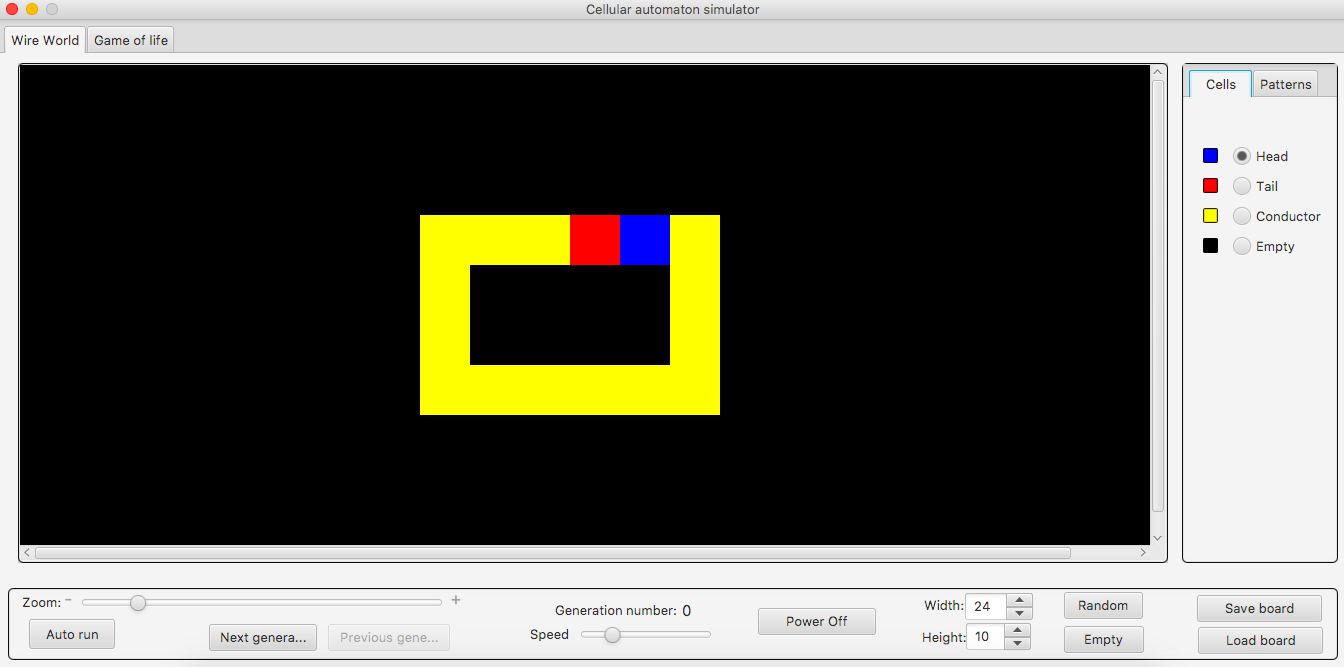
\includegraphics[width=9cm]{Obrazy/wireworld.png}
	\caption{2.1 -- GUI WireWorld}
	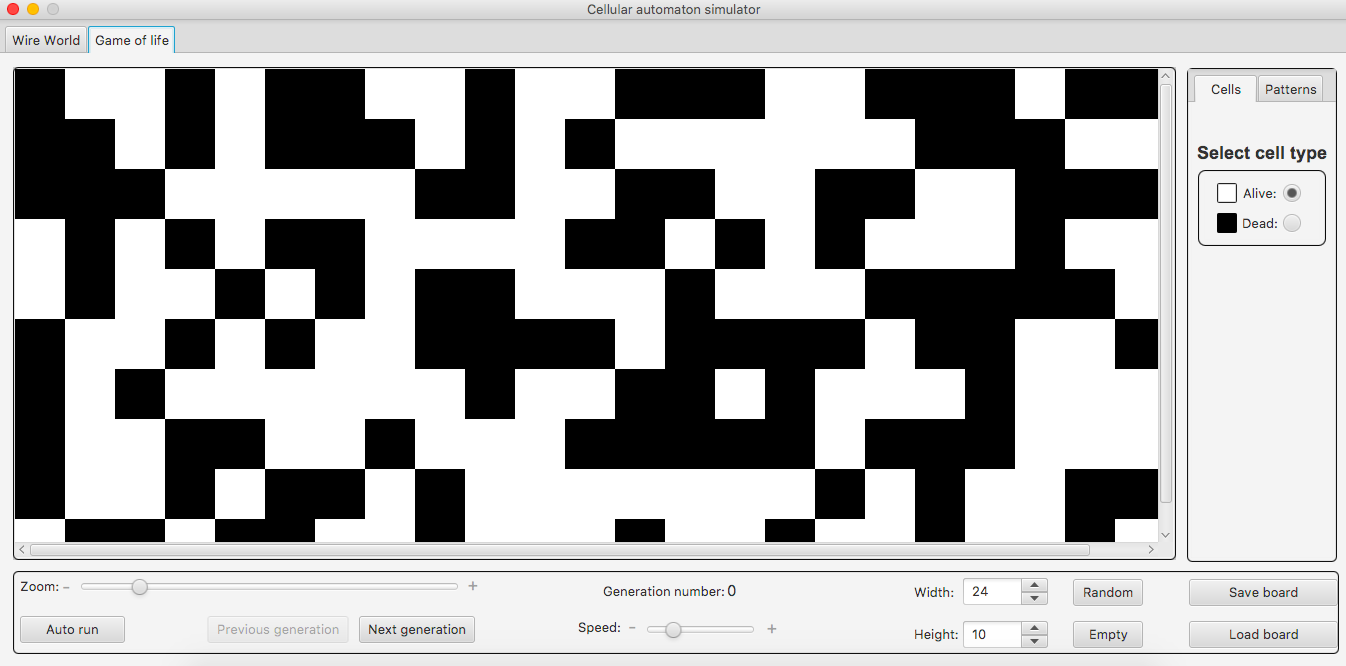
\includegraphics[width=9cm]{Obrazy/gameoflife.png}
	\caption{2.2 -- GUI GameOfLife}
	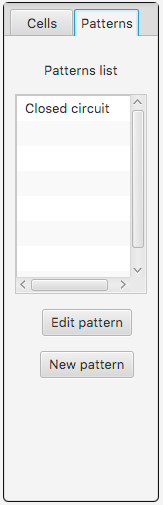
\includegraphics[width=2.5cm]{Obrazy/patterns.png}
	\caption{2.3 -- Zakładka ,,Patterns'' z bocznego menu}
	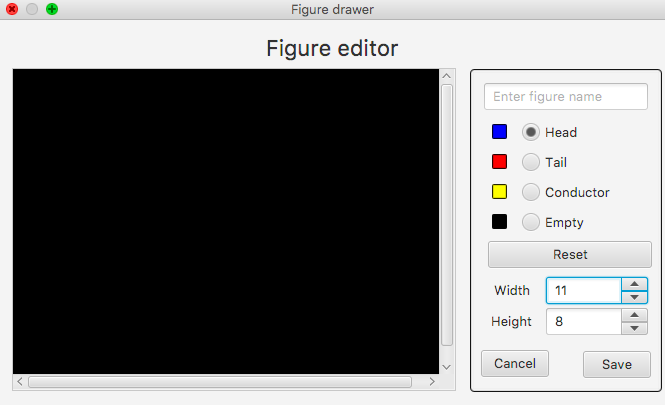
\includegraphics[width=5cm]{Obrazy/patternseditor.png}
	\caption{2.4 -- Edytor wzorów}
\end{figure}

\paragraph{Elementy wspólne interfejsów obydwu automatów:}
\begin{itemize}
	\item przycisk ,,Next generation'' -- przycisk generujący następne pokolenie,
	\item przycisk ,,Previous generation'' -- przycisk wracający do poprzedniej generacji,
	\item przycisk ,,Auto run'' -- przycisk włączający tryb automatycznej generacji kolejnych pokoleń,
	\item suwak ,,Zoom'' -- suwak pozwalający przybliżyć lub oddalić widoczną na ekranie planszę,
	\item suwak ,,Speed'' -- suwak pozwalający zmienić tempo automatycznej generacji następnych pokoleń,
	\item przycisk ,,Random'' -- przycisk odpowiedzialny za stworzenie losowo wygenerowanej planszy,
	\item przycisk ,,Empty'' -- przycisk odpowiedzialny za stworzenie pustej planszy,
	\item pole ,,Width'' -- pole reprezentujące szerokość generowanej planszy,
	\item przycisk ,,Height'' -- pole reprezentujące wysokość generowanej planszy,
	\item przycisk ,,Save board '' -- przycisk odpowiedzialny za rozpoczęcie procesu zapisu planszy,
	\item przycisk ,,Load board '' -- przycisk odpowiedzialny za rozpoczęcie procesu wczytywania planszy z odpowiedniego pliku,
	\item ,,generation number'' -- liczba reprezentująca numer aktualnie wyświetlanego pokolenia,
	\item plansza wyświetlająca aktualny stan automatu,
	\item zakładka ,,Patterns'' w panelu bocznym:
	\begin{itemize}
		\item lista dostępnych figur,
		\item przycisk ,,New pattern'' -- przycisk odpowiedzialny za otwarcie okna służącego do tworzenie nowego wzoru,
		\item przycisk ,,Edit pattern'' -- przycisk odpowiedzialny za otwarcie okna służącego do edycji istniejącego wzoru.
	\end{itemize}
\end{itemize}

\paragraph{Elementy właściwe dla automatu GameOfLife:}
\begin{itemize}
	\item pole ,,DEAD'' -- stan ,,pędzla'' -- rysowane będą komórki martwe,
	\item pole ,,ALIVE'' -- stan ,,pędzla'' -- rysowane będą komórki żywe.
\end{itemize}

\paragraph{Elementy właściwe dla automatu WireWorld:}
\begin{itemize}
	\item pole ,,TAIL'' -- stan ,,pędzla'' -- rysowane będą komórki reprezentujące ogon elektronu,
	\item pole ,,HEAD'' -- stan ,,pędzla'' -- rysowane będą komórki reprezentujące głowę elektronu,
	\item pole ,,CONDUCTOR'' -- stan ,,pędzla'' -- rysowane będą komórki reprezentujące przewodnik,
	\item pole ,,EMPTY'' -- stan ,,pędzla'' -- rysowane będą komórki puste,
	\item przycisk ,,Power off'' -- przycisk odpowiedzialny za zamianę wszystkich głów oraz ogonów elektronu w przewodniki.
\end{itemize}

\paragraph{Edytor wzorów:}
\begin{itemize}
	\item plansza służąca do narysowania wzoru,
	\item pole służące do nazwania wzorca,
	\item przycisk ,,Reset'' -- przycisk służący do zresetowania planszy,
	\item przycisk ,,Save'' -- przycisk służący do zapisania wzorca,
	\item przycisk ,,Cancel'' -- przycisk służący do anulowania procesu edycji lub tworzenia wzorca oraz do zamknięcia okna,
	\item pole ,,Width'' -- pole reprezentujące szerokość tworzonego wzorca,
	\item przycisk ,,Height'' -- pole reprezentujące wysokość tworzonego wzorca.
\end{itemize}

\section{Wzorce projektowe}
Zastosowanie wzorców projektowych nadało wyraźną strukturę projektowy. Szczególnie istotny wpływ na postać projektu miał wzorzec MVC. Dzięki niemu łatwo było wprowadzić nieprzewidziane na poprzednim etapie elementy związanie z edycją figur.

\subsection{Nowe wzorce}
W trakcie pracy nad projektem oraz poznawania przez nas większej liczby wzorców doszliśmy do wniosku, że należy skorzystać ze wzorców nieprzewidzianych w \textit{Specyfikacji Implementacyjnej}.

\paragraph{Stan} \mbox{} \\
Ponieważ główne okno symulacji udostępnia możliwość wstawiania figur jak i rysowania poszczególnych komórek za pomocą klikania widoku automatu myszą należało wyróżnić te dwie sytuacje. 
W tym celu został zastosowany wzorzec \textit{Stan}. \texttt{CellularAutomatonController} może znajdować się w stanie rysowania komórek lub wstawiania figur i w zależności od swojego stanu inaczej zareaguje na kliknięcie myszą.

\paragraphnl{Strategia}
Podczas pisania klasy \texttt{FigureEditorController} okazało się, że sporo z jej zachowań jest wspólnych z klasą \texttt{CellularAutomatonController}. By zenkapsulować te zachowania i ograniczyć duplikację kodu można by skorzystać ze wzorca \textit{Strategii}.

Niestety nie mamy doświadczenia w korzystanie z tego wzorca i nie wystarczyło czasu na jego wprowadzenie. Przy refaktoryzacji należałoby wprowadzić ten wzorzec.

\section{Potencjalna rozbudowa -- dodanie nowego automatu komórkowego}
Schemat postępowania w celu dodania nowego automatu komórkowego:
\begin{itemize}
	\item stworzyć nową kartę interfejsu graficznego w pliku \texttt{mainWindow.fxml} zawierającą sterowanie właściwego dla dodawanego automatu,
	\item zaimplementować kontroler dla danego automatu,
	\item zaimplementować model logiczny działania danego automatu,
	\item połączyć kontroler i model automatu,
	\item utworzyć pola będące referencjami do elementów interfejsu graficznego z pliku \textbf{*.fxml}, 
	\item utworzyć obiekt modelu automatu w metodzie initialize klasy SetupController
	\item \textbf{potencjalnie: } zaimplementować edytor figur dla danego automatu.
\end{itemize}

\subsection{Dodanie modelu nowego automatu}
Dzięki wykorzystaniu typów szablonowych dodanie modelu nowego automatu jest bardzo proste.
W tym celu należy:

\begin{enumerate}
	\item Utworzyć typ wyliczeniowy reprezentujący możliwe stany automatu,
	\item Rozszerzyć klasę \texttt{CellularAutomaton} konkretyzując T jako typ wyliczeniowy stanów automatu,
	\item Napisać metodę zwracającą stan następnego pokolenia na podstawie aktualnego,
	\item Uzupełnić metody pomocnicze takie jak zwracanie losowego stanu.
\end{enumerate}

Ponieważ większość zachowań jest realizowanych przez klasę abstrakcyjną \texttt{CellularAutomaton} tworzenie nowych automatów sprowadza się tylko do opisania jak będą generowane następne pokolenia.

Dzięki temu, że jest to odpowiedzialność automatu a nie poszczególne komórki możliwe są automaty delegujące generację następnego stanu do swoich komórek oraz niesymetryczne automaty, których stan następnego pokolenia może zależeć od czynników zewnętrznych.

\section{Zmiana interfejsu programu}
W związku z faktem, iż modele automatów komórkowych są niezależne od interfejsu użytkownika, można ich używać w połączeniu z dowolnym innym interfejsem -- inną biblioteką graficzną, trybem wsadowym itp. Sposób działania tych modeli opisany jest w specyfikacji implementacyjnej. Zmiany pozwalające na współpracę modeli z Parserm i Serializerem plików typu JSON lub XML -- wyżej w tym dokumencie.

\section{Podsumowanie testów jednostkowych}


\end{document}


